\section{Bestimmen des Rollreibungskoeffizienten}
Rollt eine Kugel einen bestimmten Weg über den Billardtisch, so entsteht eine Reibungskraft, welche der
Geschwindigkeit entgegengesetzt wirkt. Die Kraft kann als negative Beschleunigung angegeben werden, wobei diese von einem
Rollreibungskoeffizienten $c_R$ oder $\mu_r$ abhängig ist. Das Finden dieses Koeffizienten wird in diesem Kapitel beschrieben.
Die Herleitung und theoretischen Überlegungen finden sich in Kapitel \ref{anhang:herleitung:reibungskoeffizient}.
Der Rollreibungskoeffizient ist für viele Berechnungen, welche im Anhang erläutert werden, notwendig.

\begin{figure}[h!]
    \begin{center}
        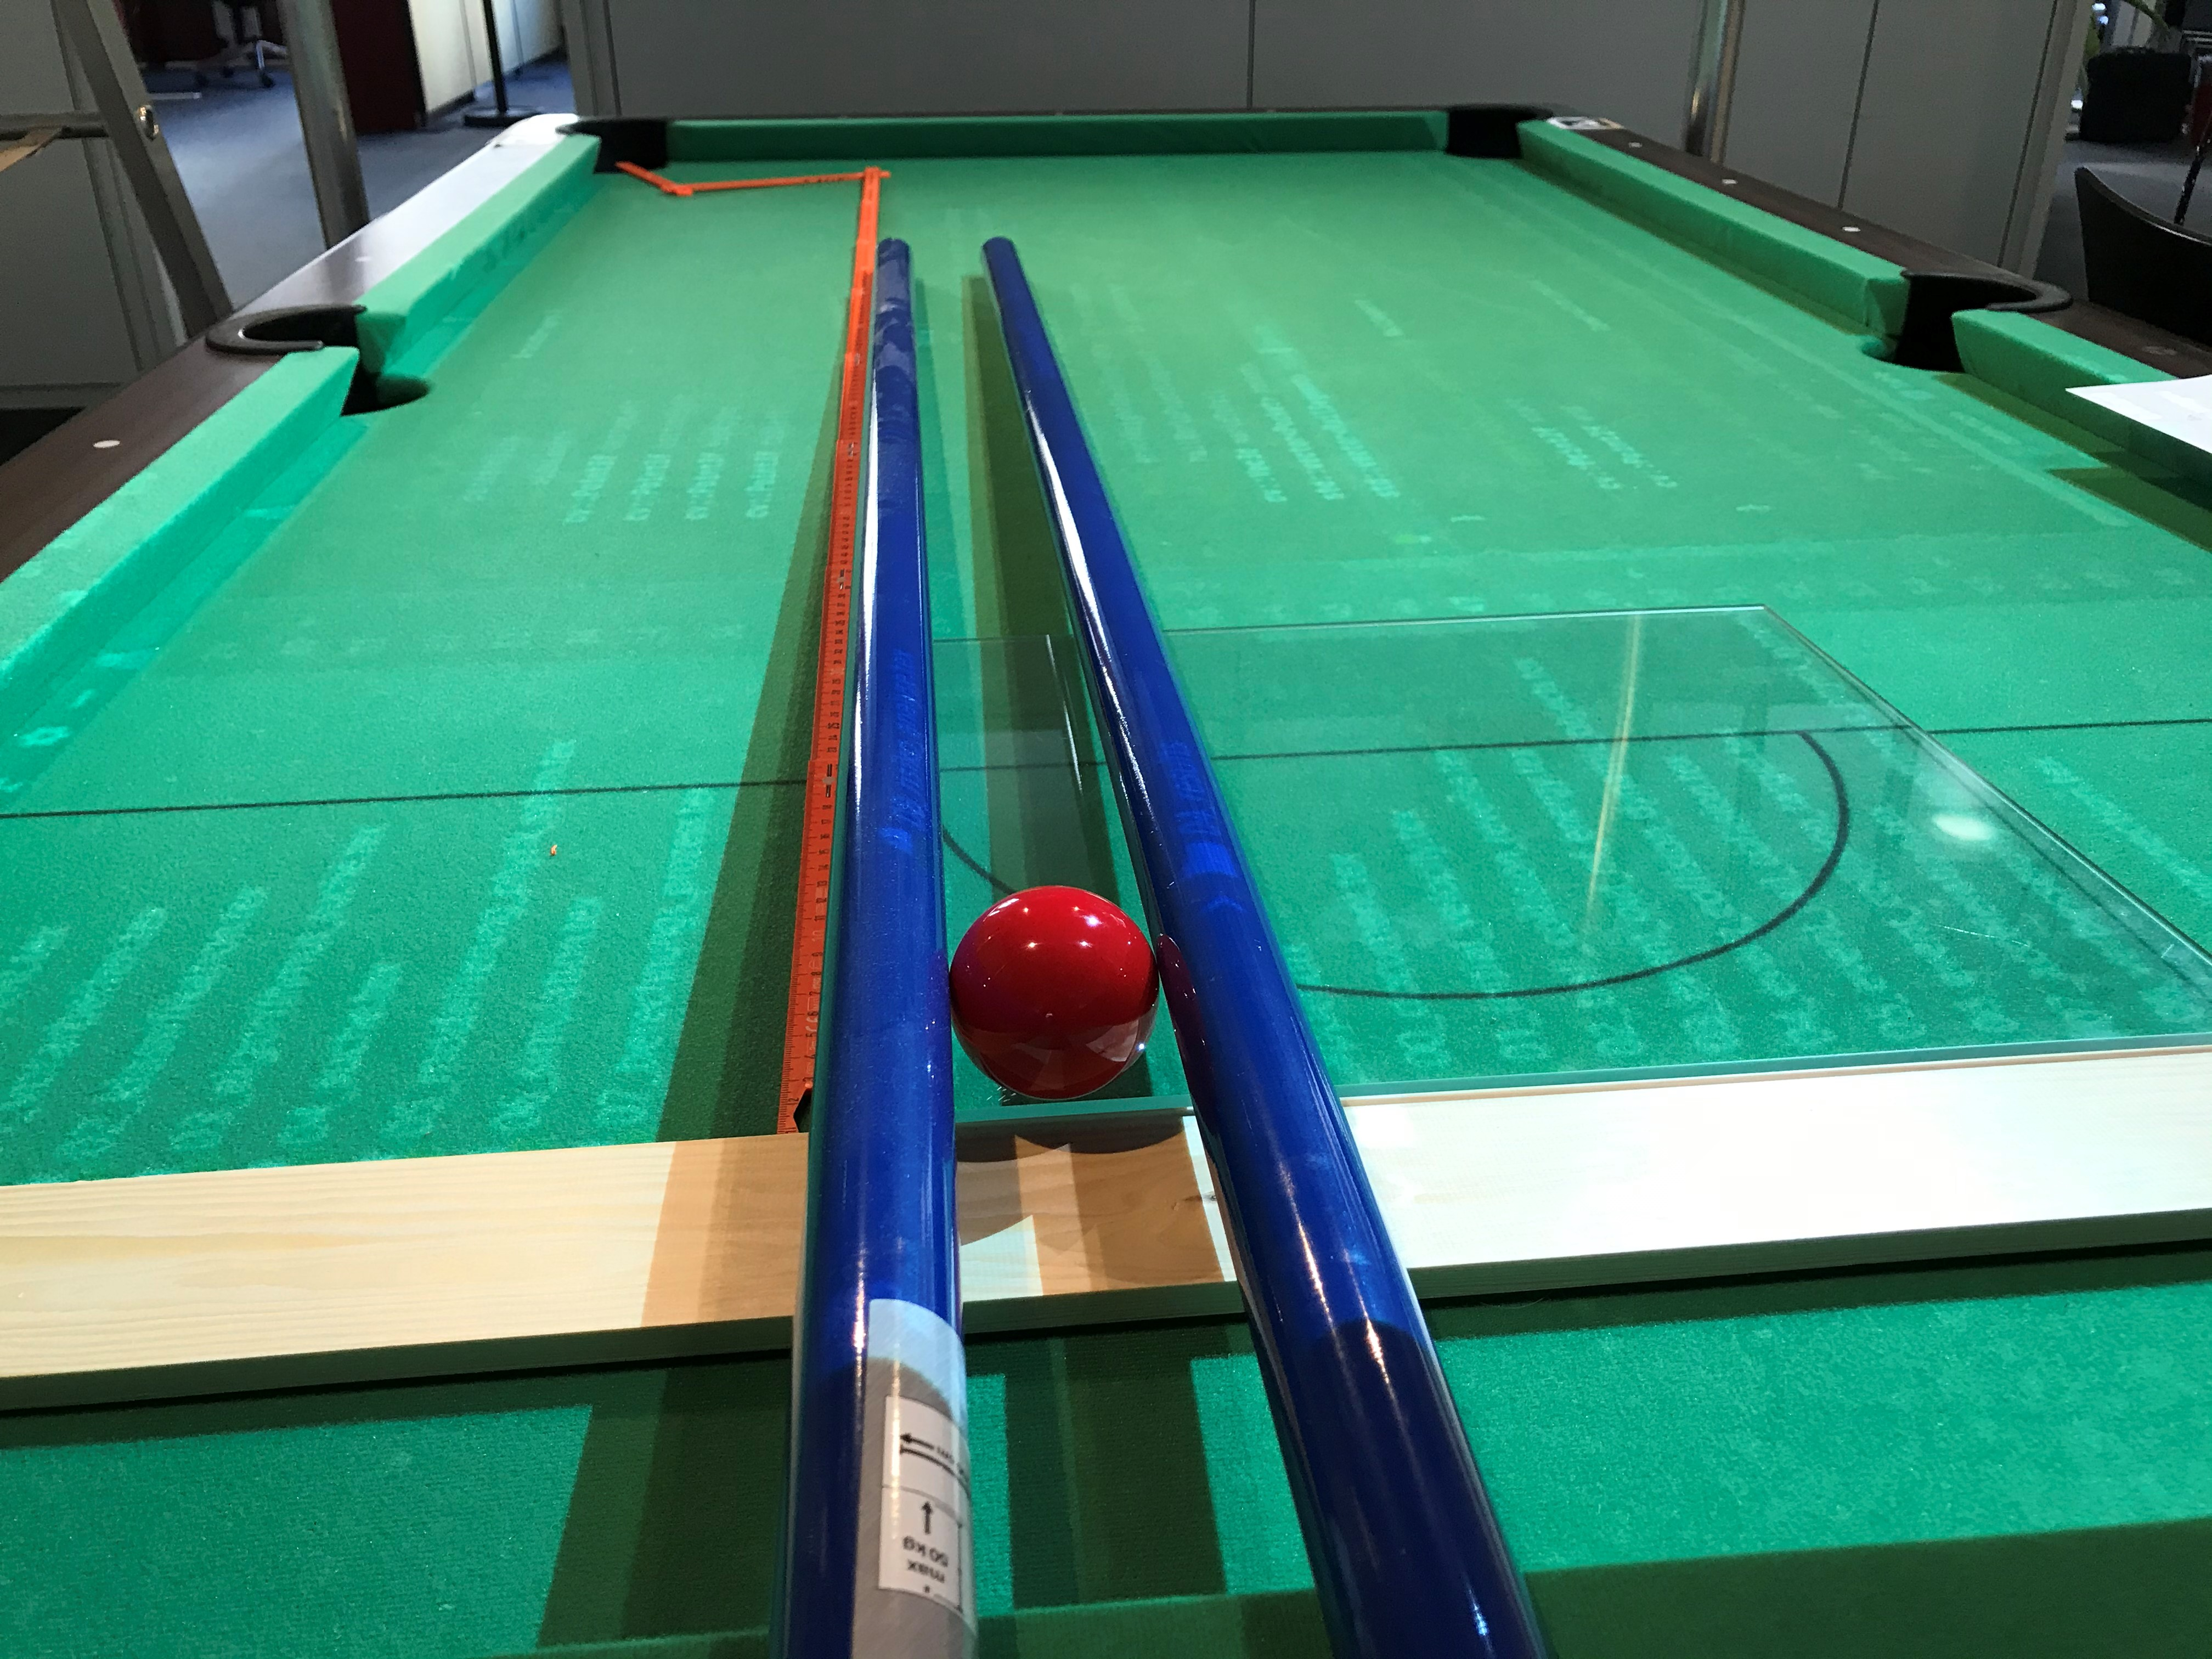
\includegraphics[width=0.5\linewidth]{../common/04_results/resources/00_versuchsaufbau_reibungskoeffizient.png}
    \end{center}
    \caption{Versuchsaufbau zur Bestimmung des Reibungskoeffizienten}
    \label{fig:versuchsaufbau_reibungskoeffizient}
\end{figure}

Abbildung \ref{fig:versuchsaufbau_reibungskoeffizient} veranschaulicht den Versuchsaufbau zur Bestimmung des
Rollreibungskoeffizienten. Wie in Kapitel \ref{anhang:herleitung:reibungskoeffizient} erläutert, muss für die
Rampe ein Material mit möglichst geringer Reibung verwendet werden, weswegen die Wahl auf Glas fiel.
Weiterhin wird der Weg der Kugel geführt, da sie eine möglichst gerade Bahn rollen muss. Die so entstehende Reibung
an der Bahn wird ebenfalls vernachlässigt.

Es wurden zwei Versuche durchgeführt mit unterschiedlicher Höhe der Rampe. Die Ergebnisse dieser Messungen wie
deren Median sind in der Tabelle \ref{tab:distanzmessungen_rollende_kugel} aufgeführt.

\begin{table}[ht]
    \rowcolors{1}{\seccolor!10}{\seccolor!10} % Rows with 10% of secondary color
    \begin{tabular}{ccc}
        \rowcolor{\seccolor!50}
        \textbf{Höhe {[}mm{]}} & \textbf{13}  & \textbf{19}\\
        & 957          & 1228\\
        & 949          & 1253\\
        & 926          & 1263\\
        & 914          & 1280\\
        & 931          & 1281\\
        & 932          & 1296\\
        & 941          & 1256\\
        & 926          & 1295\\
        & 931          & 1295\\
        & 941          & 1304\\
        & 943          & 1314\\
        & 937          & 1316\\
        & 947          & 1284\\
        & 949          & 1303\\
        & 947          & 1319\\
        \multirow{-16}{*}{\rotatebox{90}{\textbf{Distanz {[}mm{]}}}} & -            & 1320\\
        \textbf{Median} & \textbf{941} & \textbf{1295}\\
    \end{tabular}
    \caption{Ergebnisse der Distanzmessungen einer Kugel, welche über eine Rampe beschleunigt wurde.}
    \label{tab:distanzmessungen_rollende_kugel}
\end{table}

Anhand des Ablaufs aus Kapitel \ref{anhang:herleitung:reibungskoeffizient} können die Reibungskoeffizienten mithilfe
der Daten aus Tabelle \ref{tab:distanzmessungen_rollende_kugel} bestimmt werden. Die Resultate sind in Tabelle
\ref{tab:reibungskoeffizienten}. Daraus wird der Mittelwert berechnet, welcher das Resultat bildet.

\begin{table}[h!t]
    \rowcolors{1}{\seccolor!10}{\seccolor!10} % Rows with 10% of secondary color
    \begin{tabular}{cc}
        \rowcolor{\seccolor!50}
        \textbf{Strecke {[}mm{]}} & \textbf{Reibungskoeffizient} \\\bfhmidline
        941                       & 0.0138151                    \\\bfhmidline
        1295                      & 0.0146718                    \\\bfhmidline
        \textbf{Mittelwert}       & 0.0142435                    \\\bfhmidline
    \end{tabular}
    \caption{Reibungskoeffizienten über Strecke}
    \label{tab:reibungskoeffizienten}
\end{table}